%%% Пример оформления определения

\emph{Фазоманипулированный сигнал} "--- это последовательность элементарных импульсов длительностью $\tau_0$, фазы сигнала в которых изменяются по определенному закону, принимая два или более фиксированных значений. При этом, если количество элементарных импульсов равно $N$, то общая длительность сигнала составляет $T=\tau_0\cdot N$. 


%%% Как ссылаемся на источник
Ширина спектра такого сигнала примерно равна~\cite{Suzev}.

%%% Как оформляем формулы 
%%% labN_eq:spectr- Имя метки состоит из двух частей, где labN - номер лабы (берем из таблицы), spectr - краткое название формулы

\begin{equation}
\Delta f= \frac{1}{\tau_0} = \frac{N}{T}.
\label{labN_eq:spectr}
\end{equation}
	
Фазоманипулированный сигнал является сложным, а его база с учетом выражения \eqref{labN_eq:spectr} определяется как $B = \Delta f \cdot T = N$.

%%% Пример с формулой без ссылки по тексту (работает правило, описанное в Лекции 2 слайд 10)
	
Опишем сигнал несущей частоты выражением

\begin{equation}
S(t) = A\cos(2\pi f t +\theta), 
\label{labN_eq:carryf}
\end{equation}
где $A$ "--- амплитуда, $f$ "--- частота, $\theta$ "--- начальная фаза несущего колебания.
   
В настоящее время известны девять последовательностей Баркера (\autoref{labN_tab:table1}), а наиболее длинная из них имеет длину $N_{max}=13$. Соотношение уровней основного и боковых лепестков автокорреляционной функции зависит от длины последовательности Баркера и равно $\displaystyle \frac{1}{N}$.

\begin{table}[H]
\caption{Последовательности Баркера}
\label{labN_tab:table1}
\begin{tabular}{|p{1.2cm}|p{4cm}|p{4cm}|}
\hline
Длина & \multicolumn{2}{c|}{Последовательности} \\ \hline
$2$ & $+1 -1$ & $+1 +1$ \\ \hline
$3$ & \multicolumn{2}{l|}{$+1 +1 -1$} \\ \hline
$4$ & $+1 -1 +1 +1$ & $+1 -1 -1 -1$ \\ \hline
$5$ & \multicolumn{2}{l|}{$+1 +1 +1 -1 +1$} \\ \hline
$7$ & \multicolumn{2}{l|}{$+1 +1 +1 -1 -1 +1 -1$} \\ \hline
$11$ & \multicolumn{2}{l|}{$+1 +1 +1 -1 -1 -1 +1 -1 -1 +1 -1$} \\ \hline
$13$ & \multicolumn{2}{l|}{$+1 +1 +1 +1 +1 -1 -1 +1 +1 -1 +1 -1 +1$} \\ \hline
\end{tabular}
\end{table} 
	
Пример интеграции изображения, полученного с помощью пакета Tikz (рисунок~\ref{labN_fig:probability}).

\begin{figure}[pt!]
	\centering
	\scalebox{.85}{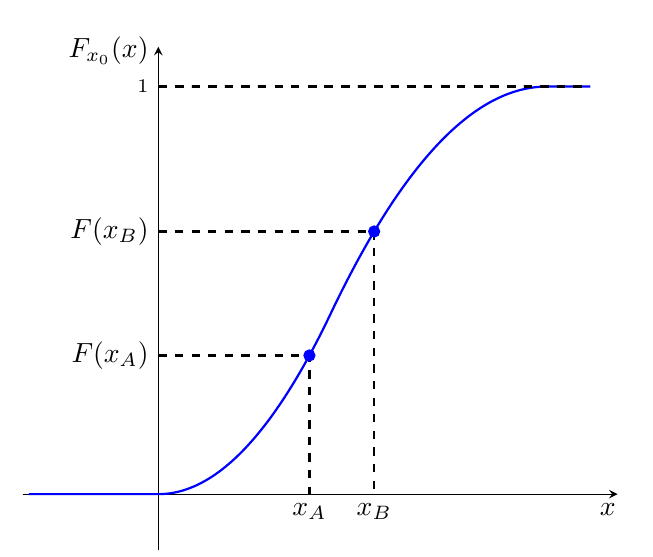
\begin{tikzpicture}[
declare function= {
    triangle(\x,\a,\b,\c) = 0+(\x<=\c)*(\x>=\a)*(pow(\x-\a,2)/((\b-\a)*(\c-\a)))+(\x<=\b)*(\x>\c)*(1-pow(\b-\x, 2)/((\b-\a)*(\b-\c)))+1*(\x>\b);
}
]
\begin{axis}[
    clip=false,
    axis lines = middle,
    axis line style={shorten >=-10pt, shorten <=-10pt},
    xlabel = {$x$}, % подпись оси x
    ylabel = {$F_{x_0}(x)$}, % подпись оси y
    xlabel style={below right},
    ylabel style={above left},	
    ymax = 1.03,
    ymin = -0.07,
    xmin = -2.5,
    xtick={0}, 
    ytick={0}
    ]
    \coordinate (a1)  at (0,{triangle(3.5, 0, 9, 4)});
    \coordinate (a2)  at (3.5,{triangle(3.5, 0, 9, 4)});
    \coordinate (a3)  at (3.5,0);
    \node at (a1) [left] {$F(x_A)$};
    \node at (a3) [below] {$x_A$};
    \draw [thick, dashed] (a1)--(a2)--(a3);
    %
    \coordinate (b1)  at (0,{triangle(5, 0, 9, 4)});
    \coordinate (b2)  at (5,{triangle(5, 0, 9, 4)});
    \coordinate (b3)  at (5,0);
    \node at (b1) [left] {$F(x_B)$};
    \node at (b3) [below] {$x_B$};
    \draw [thick, dashed] (b1)--(b2)--(b3);
    %
    \addplot[domain=-3:10, samples=300, color=blue, thick] {triangle(x, 0, 9, 4)};
    %\addplot[blue,samples=200]{triangle(x, 0, 9, 4)};
    \addplot[blue, only marks,samples at={3.5,5}]{triangle(x, 0, 9, 4)};
    \addplot[domain=0:10, samples=300, color=black, thick, dashed] {1};
    \coordinate (c1)  at (0,1);
    \node at (c1) [left] {\scriptsize $1$};
\end{axis}
\end{tikzpicture}}
	\caption{Пример функции распределения непрерывной случайной величины}
	\label{labN_fig:probability}
\end{figure}

%%% Далее идет пример оформления ненумерованного списка. Поскольку файл стиля перегружен, то пришлось вводить костыль
	
М"~последовательности обладают следующими основными свойствами:	
\renewcommand{\labelitemi}{--}
\begin{itemize}
    \item М"~последовательности являются периодическими с периодом $M=2^n-1$, где $n$"--- порядок порождающего полинома $h(x)$;
    \item количество символов, принимающих значение единица, на длине одного периода М"~последовательности на единицу больше, чем количество символов, принимающих значение ноль;
    \item сумма по модулю $2$ любой М"~последовательности с её произвольным циклическим сдвигом также является М"~последовательностью;
    \item периодическая автокорреляционная функция любой М"~последовательности имеет соотношение уровней основного и боковых лепестков, равное $\displaystyle\frac{1}{M}$;
    \item автокорреляционная функция усечённой М"~последовательности (непериодическая последовательность длиной, соответствующей периоду $M$) имеет соотношение уровней основного и боковых лепестков, близкое к $\displaystyle\frac{1}{\sqrt{M}}$.
\end{itemize}
\vspace{10mm}